\setcounter{section}{8}
\section{Теория меры}

\subsection{Система множеств}

\subsubsection*{Обозначение:}

\textit{Дизъюнктные множества:} 
\begin{enumerate}
    \item $A \sqcup B := A \cup B$ и $A \cap B = \varnothing$
    \item $\bigsqcup\limits_{k=1}^n A_k := \bigcup\limits_{k=1}^n A_k$ и $A_i \cap A_j = \varnothing$
\end{enumerate}

\begin{definition}
    $\{E_\alpha\}_{\alpha\in I}$ – \textit{разбиение множества $E$}, если $E = \bigsqcup\limits_{\alpha\in I} E_\alpha$
\end{definition}

\subsubsection*{Напоминание:}

$X \setminus  \bigcup\limits_{\alpha \in I} E_\alpha = \bigcap\limits_{\alpha \in I} (X\setminus E_\alpha)$ и 
$X \setminus  \bigcup\limits_{\alpha \in I} E_\alpha = \bigcap\limits_{\alpha \in I} (X\setminus E_\alpha)$

\begin{definition}
    $\mathcal{A}$ – система подмножеств $X$:
    \begin{enumerate}
        \item[$\delta_0$.] Если $A, B\in \mathcal{A}$, то $A\cap B\in \mathcal{A}$.
        \item[$\sigma_0$.] Если $A, B\in \mathcal{A}$, то $A\cup B\in \mathcal{A}$.
        \item[$\delta$.] Если $A_1, A_2, ...\in \mathcal{A}$, то $\bigcap\limits_{n = 1}^\infty A_n\in \mathcal{A}$.
        \item[$\sigma$.] Если $A_1, A_2, ...\in \mathcal{A}$, то $\bigcup\limits_{n = 1}^\infty A_n\in \mathcal{A}$.
    \end{enumerate}
\end{definition}

\begin{remark}
    Из $\delta$ следует $\delta_0$ и из $\sigma$ следует $\sigma_0$ (так как $\delta$ и $\sigma$ подразумевают 
    более сильные ограничения на структуру).
\end{remark}

\begin{definition}
    Система множества \textit{симметрична}, если $A\in \mathcal{A}\Rightarrow X\setminus A\in \mathcal{A}$.
\end{definition}

\begin{definition}
    Система множества $\mathcal{A}$ – \textit{алгебра}, если она симметрична, $\varnothing \in \mathcal{A}$, есть свойства $\delta_0$ и $\sigma_0$.
\end{definition}

\begin{definition}
    Система множества $\mathcal{A}$ – \textit{$\sigma$-алгебра}, если она симметрична, $\varnothing \in \mathcal{A}$, есть свойства $\delta$ и $\sigma$.
\end{definition}

\begin{statement}
    Если $\mathcal{A}$ симметричная система, то $\sigma_0\Leftrightarrow \delta_0$ и $\sigma\Leftrightarrow \delta$.
\end{statement}

\begin{proof}
    $X\setminus (\underbrace{(X\setminus A)\cup (X\setminus B)}_{X\setminus (A\cap B)})= A\cap B\quad\text{и}\quad
    X\setminus (\underbrace{(X\setminus A)\cap (X\setminus B)}_{X\setminus (A\cup B)})= A\cup B$
\end{proof}

\begin{remark}
    Если $\mathcal{A}$ – $\sigma$-алгебра, то $\mathcal{A}$ – алгебра.
\end{remark}

\subsubsection*{Свойства алгебры множеств:}

\begin{enumerate}
    \item $\varnothing, X\in \mathcal{A}$.
    \item Если $A, B \in \mathcal{A}$, то $\underbrace{A\setminus B}_{A\cap (X \setminus B)}\in \mathcal{A}$.
    \item Если $A_1, A_2, ..., A_n\in \mathcal{A}$, то $\bigcup\limits_{k = 1}^n A_k$ и $\bigcap\limits_{k = 1}^n A_k\in \mathcal{A}$ (по индукции).
\end{enumerate}

\begin{example} 
    \begin{enumerate}
        \item[]
        \item $X=\R^2$, $\mathcal{A} = \{\text{все огранич. мн-ва и их дополнения}\}$
        
        (пустое есть, для любого множества есть дополнение, пересечение двух ограниченных ограниченно,
        пересечение ограниченного с каким-то ограничено и пересечение дополнений – это дополнение объединений, а 
        объединение ограниченных ограничено)
        
        $\mathcal{A}$ – алгебра, но не $\sigma$-алгебра.

        \item $2^X$ – $\sigma$-алгебра
        
        \item $Y\subset X$, $\mathcal{A}$ – алгебра ($\sigma$-алгебра) подмножеств $X$, тогда:
        
        $\mathcal{B} := \{ A\cap Y \mid A\in \mathcal{A}\}$ – алгебра ($\sigma$-алгебра) – \textit{индуцированная алгебра}

        \begin{proof}
            $Y \setminus (A\cap Y) = Y \cap (X \setminus A)$

            Проверили, что взяли какую-то алгберу и пересекли с конкретным множеством, то структура сохранится.

            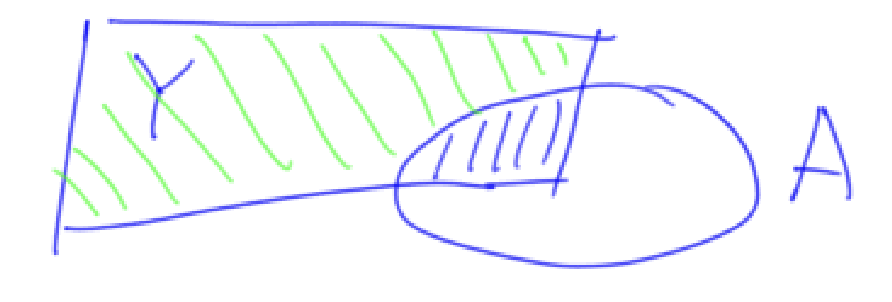
\includegraphics[width=0.3\linewidth]{images/23-09-07-1.png}
        \end{proof}

        \item Пусть $\mathcal{A}_\alpha$ – алгебры ($\sigma$-алгебры). Тогда $\bigcap\limits_{\alpha \in I} \mathcal{A}_\alpha$ – алгебра ($\sigma$-алгебра).
        
        \begin{proof}
            Пустое лежало везде, поэтому оно осталось в пересечении. Само пересечение, очевидно, тоже есть.

            Если $A, B\in \bigcap\limits_{\alpha \in I} A_\alpha$, то $A, B\in \mathcal{A}_\alpha\ \forall \alpha \in I\Rightarrow A\cup B \in \mathcal{A}_\alpha\ \forall \alpha \in I\Rightarrow \bigcap\limits_{\alpha \in I} A_\alpha$
        \end{proof}

        \item Пусть есть $A, B\subset X$. 
        
        \textit{Вопрос:} из чего состоит наименьшая алебра, содержащая $A$ и $B$?
        
        \textit{Ответ:} $\varnothing, X, A, B, A\cap B, A \cup B, X \setminus A,  X \setminus B,  X \setminus (A\cap B),  X \setminus (A\cup B), A\setminus B, B\setminus B,$
        
        $A\triangle B, X \setminus (A\triangle B), X\setminus (A\setminus B), X\setminus (B\setminus A)$

        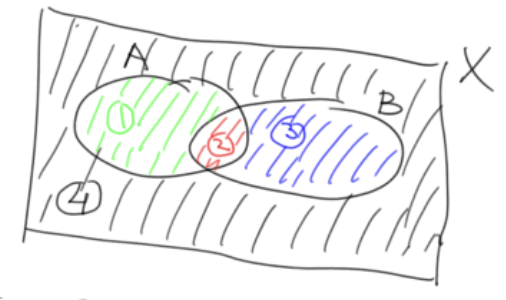
\includegraphics[width=0.3\linewidth]{images/23-09-07-2.png}
    \end{enumerate}
\end{example}

\begin{theorem}
    Пусть $\mathcal{E}$ – система подмножеств $X$. Тогда существует наименьшая по включению $\sigma$-алгебра $\mathcal{A}$,
    содержащая $\mathcal{E}$.
\end{theorem}

\begin{proof}
    $2^X$ – $\sigma$-алгебра, содержащая $\mathcal{E}$.

    Пусть $\mathcal{A}_\alpha$ – всевозможные $\sigma$-алгебры, содержащие $\mathcal{E}$.

    $\mathcal{B} :=\bigcap\limits_{\alpha \in I}\mathcal{A}_\alpha$ – $\sigma$-алгебра, $\mathcal{B} \supset \mathcal{E}$ и $\mathcal{A}_\alpha \supset \mathcal{E}\ \forall \alpha$.

    Доказали сущестование.
\end{proof}

\begin{definition}
    Такая $\sigma$-алгебра – \textit{борелевская оболочка $\mathcal{E}$}. Обозначается как $\mathcal{B}(\mathcal{E})$.
\end{definition}

\begin{definition}
    Пусть $X=\R^m$, $\mathcal{E}$ – всевозможные открытые множества. \textit{Борелевская $\sigma$-алгебра} $\mathcal{B}^m:=\mathcal{B}(\mathcal{E})$.
\end{definition}

\begin{remark}
    $\mathcal{B}^m\not = 2^{\R^m}$ (имеют разные мощности: $\mathcal{B}^m$ – континуум, $2^{\R^m}$ – больше континуума)
\end{remark}

\begin{definition}
    $\mathcal{R}$ – \textit{кольцо подмножеств $X$}, если $A, B\in \mathcal{R}\Rightarrow A \cap B,  A \cup B,  A \setminus B\in \mathcal{R}$
\end{definition}

\begin{remark}
    Если $\mathcal{R}$ – кольцо и $X\in \mathcal{R}$, то $\mathcal{R}$ – алгебра.
\end{remark}

\begin{definition}
    $\mathcal{P}$ – \textit{полукольцо подмножеств $X$}, если:
    \begin{enumerate}
        \item $\varnothing \in \mathcal{P}$
        \item $A, B \in \mathcal{P}\Rightarrow A \cap B \in \mathcal{P}$
        \item $A, B \in \mathcal{P}\Rightarrow$ существуют $Q_1, Q_2, ..., Q_n\in \mathcal{P}$ 
            т.ч. $A\setminus B =\bigsqcup\limits_{k=1}^n Q_k$
    \end{enumerate}
\end{definition}

\begin{example}
    $X=\R$, $\mathcal{P}:=\{ (a, b] \mid a, b\in \R\}$ – полукольцо

    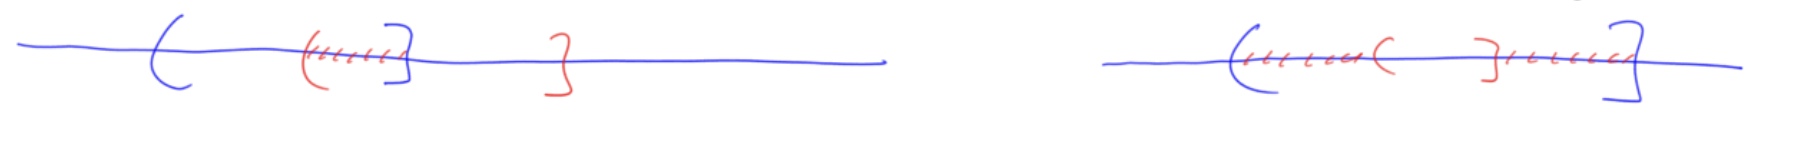
\includegraphics[width=0.7\linewidth]{images/23-09-07-3.png}
\end{example}

\begin{lemma}
    $\bigcup A_k=\bigsqcup (A_k \setminus \bigcup\limits_{j=1}^{k - 1} A_j)$ 
\end{lemma}

\begin{proof} Проверяем «$\supset$»: $B_k := A_k \setminus \bigcup\limits_{j=1}^{k-1} A_j \subset A_k \Rightarrow \bigcup A_k \supset \bigcup B_k$

    Проверяем, что $B_k$ дизъюнктны: $B_n \subset A_n \setminus \underbrace{A_k}_{\supset B_k}$ при $n>k\Rightarrow B_n \cup B_k = \varnothing$

    Проверяем «$\subset$»: берем $x\in \bigcup A_k$, $n:=\min \{j\mid x\in A_j\}\Rightarrow x\in B_n=\underbrace{A_n}_{x\in}\setminus \underbrace{\bigcup\limits_{j=1}^{n-1} A_j}_{x\not\in} 
    \Rightarrow x\in \bigcup B_k$.
\end{proof}

\begin{theorem}
    \textbf{Свойства полукольца:}

    Пусть $P, P_1, P_2, ... \in \mathcal{P}$, где $\mathcal{P}$ – полукольцо. Тогда:
    \begin{enumerate}
        \item $P\setminus \bigcup\limits_{k=1}^n P_k= \bigsqcup\limits_{j=1}^m Q_j$ для некоторых $Q_j\in \mathcal{P}$.
        \item $\bigcup\limits_{k=1}^n P_k=\bigsqcup\limits_{k=1}^n \bigsqcup\limits_{j=1}^{m_k} Q_{kj}$ для некоторых $Q_{kj}\in \mathcal{P}$, т.ч. $Q_{kj}\subset P_k$.
        \item Во 2 пункте можно вместо $n$ написать $\infty$.
    \end{enumerate}
\end{theorem}

\begin{proof}~
    \begin{enumerate}
        \item Индукция по $n$. База – определение. Переход $n -1 \rightarrow n$
        
        $P \setminus \bigcup\limits_{k=1}^n P_k = (\underbrace{P \setminus \bigcup\limits_{k=1}^{n-1} P_k}_{\text{инд.пр.} = \bigsqcup\limits_{j=1}^m Q_j}) 
        \setminus P_n=\bigsqcup\limits_{j=1}^m Q_j \setminus P_n = \bigsqcup\limits_{j=1}^m\bigsqcup\limits_{i=1}^{m_j} Q_{ji}$

        \item $\bigcup\limits_{k=1}^n P_k = \bigsqcup\limits_{k=1}^n (P_k \setminus \bigcup\limits_{j=1}^{k -1} P_j)\overset{\text{по 1}}{=}\bigsqcup\limits_{k=1}^n \bigsqcup\limits_{j=1}^{m_k}Q_{kj}\Rightarrow Q_{kj}\subset P_k$
    \end{enumerate}
\end{proof}

\begin{theorem}
    \textbf{Декартово произведение полуколец}

    Пусть $\mathcal{P}$ – полукольцо подмножеств мн-ва $X$, $\mathcal{Q}$ – полукольцо подмножеств мн-ва $Y$.

    Тогда конструкция $\mathcal{P}\times \mathcal{Q} := \{ P\times Q \mid P \in \mathcal{P}, Q\in \mathcal{Q}\}$ – полукольцо подмножеств $X\times Y$.
\end{theorem}

\begin{proof}
    Пусть $P_1\times Q_1$ и $P_2\times Q_2\in \mathcal{P}\times \mathcal{Q}\Rightarrow (P_1\times Q_1) \cap (P_2\times Q_2)=(\underset{\in \mathcal{P}}{P_1\cap P_2})\times \underset{\in \mathcal{Q}}{(Q_1\cap Q_2)}$

    $(P_1\times Q_1) \setminus (P_2\times Q_2)= (\underset{\text{диз. об. эл-в }\mathcal{P}}{P_1 \setminus P_2}) \times \underset{\in \mathcal{Q}}{Q_1} \sqcup ( \underset{\in \mathcal{P}}{P_1\cap P_2}) \times (\underset{\text{диз. об. эл-в }\mathcal{Q}}{Q_1\setminus Q_2})$

    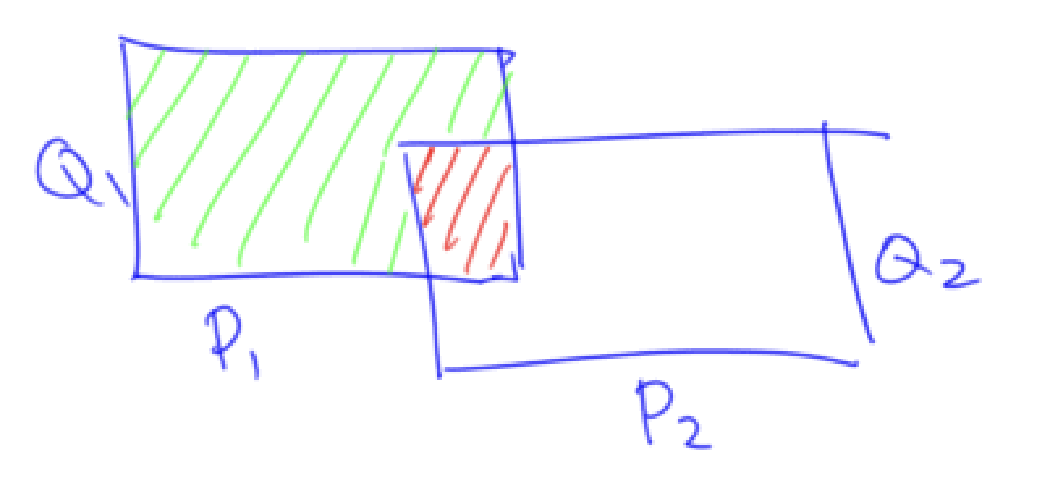
\includegraphics[width=0.3\linewidth]{images/23-09-07-4.png}
\end{proof}

\begin{remark}
    Полукольцо – это структура, которая сохраняется при взятии декартового произведения (в отличие 
    от алгебры и $\sigma$-алгебры).
\end{remark}

\begin{definition}
    \textit{Открытый параллелепипед $(a, b)$}, $a, b\in \R^m$

    $(a, b):= (a_1, b_1)\times (a_2, b_2)\times ...\times (a_m, b_m)$
\end{definition}

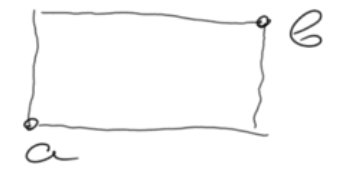
\includegraphics[width=0.2\linewidth]{images/23-09-07-5.png}

\begin{definition}
    \textit{Замкнутый параллелепипед $[a, b]$}, $a, b\in \R^m$

    $[a, b]:= [a_1, b_1]\times [a_2, b_2]\times ...\times [a_m, b_m]$
\end{definition}

\begin{definition}
    \textit{Ячейка $(a, b]$}, $a, b\in \R^m$

    $(a, b]:= (a_1, b_1]\times (a_2, b_2]\times ...\times (a_m, b_m]$
\end{definition}

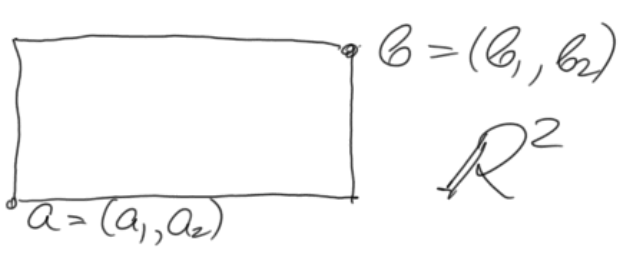
\includegraphics[width=0.3\linewidth]{images/23-09-07-6.png}

\begin{remark}
    $(a, b)\subset (a, b]\subset [a, b]$
\end{remark}

\begin{statement}
    Непустая ячейка – пересечение убывающей последовательности открытых параллелепипедов
    и объединение возрастающих последовательностей замкнутых параллелепипедов.
\end{statement}

\begin{proof}
    $(a, b] = (a_1, b_1] \times (a_2, b_2] \times ... \times (a_m, b_m]$

    Рассмотрим открытые параллелепипеды $P_n:=(a_1, b_1 +\frac{1}{n})\times (a_2, b_2 +\frac{1}{n})\times ...\times (a_m, b_m +\frac{1}{n})$

    $P_{n+1}\subset P_n$, $P_n\supset (a, b]$ и $\bigcap\limits_{n=1}^\infty P_n=(a, b]$

    Рассмотрим закрытые параллелепипеды $A_n := [a_1 - \frac{1}{n}, b_1] \times [a_2 - \frac{1}{n}, b_2] \times .. \times [a_m - \frac{1}{n}, b_m]$

    $A_{n+1} \supset A_n \subset (a, b]$, $\bigcup A_n = (a, b]$

    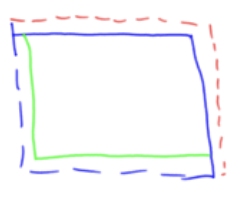
\includegraphics[width=0.18\linewidth]{images/23-09-07-7.png}
\end{proof}

\textbf{Обозначение:} 
\begin{enumerate}
    \item $\mathcal{P}^m$ – семейство ячеек в $\R^m$ (в т.ч. и пустое множество).
    \item $\mathcal{P}_{\Q}^m$ – семейство ячеек в $\R^m$, у которых все координаты вершин рациональны.
\end{enumerate}

\begin{theorem}
    Всякое непустое открытое множество $G \subset \R^m$ представляется в виде дизъюнктного объединения
    счетного числа ячеек, замыкания которых $\subset G$. Более того, можно считать, что координаты всех 
    вершин всех ячеек рациональны.
\end{theorem}

\begin{proof}
    $x\in G\overset{G\text{ откр.}}{\Rightarrow} x\in \overline{\text{B}}_{r}(x)\subset G$

    Найдется ячейка $R_x$, т.ч. $x\in R_x$, координаты $R_x$ рациональны и $\Cl R_x \subset G$ ($\Cl$ содержится
    в $\overline{\text{B}}_{r}(x)$, которое содержится в $G$). 
    
    Выкинем все повторы и получим счетное число ячеек, объединение которых (не дизъюнктное) равно $G$. По свойству 
    полукольца можно это объединение сделать дизъюнктным.

    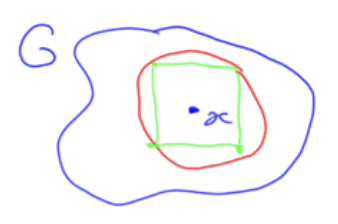
\includegraphics[width=0.2\linewidth]{images/23-09-07-8.png}
\end{proof}

\begin{remark}
    Явный алгоритм.
\end{remark}

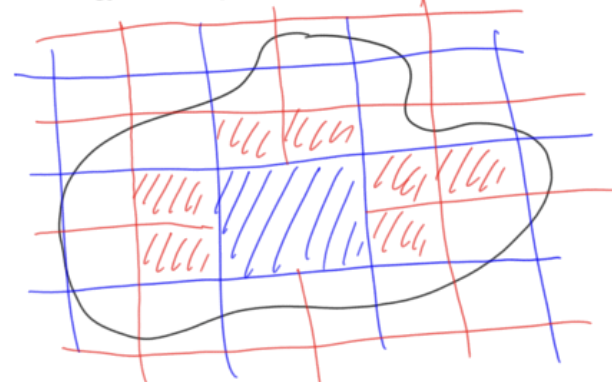
\includegraphics[width=0.2\linewidth]{images/23-09-07-9.png}

Нарезаем на сетку. Те ячейки, которые попали – берем, иначе – половинем и снова смотрим, какие из ячеек попали, а какие нет.  

\begin{corollary}
    $\mathcal{B}(\mathcal{P}_{\Q}^m)\overset{1) \subset}{=} \mathcal{B}(\mathcal{P}^m)\overset{2) \subset}{=}\mathcal{B}^m \overset{3) \subset}{=}$
\end{corollary}

\begin{proof}~
    \begin{enumerate}
        \item[1)] $\mathcal{P}^m\supset \mathcal{P}^m_\Q\Rightarrow \mathcal{B}(\mathcal{P}^m)\supset \mathcal{P}^m_\Q\overset{\sigma\text{-алгебра}}{\Rightarrow} \mathcal{B}(\mathcal{P}^m)\supset \mathcal{B}(\mathcal{P}^m_\Q)$
        \item[2)] $\mathcal{P}^m \subset \mathcal{B}^m\Rightarrow \mathcal{B}(\mathcal{P}^m)\subset \mathcal{B}^m$

        Ячейка – счетное пересечение открытых параллелепипедов, т.е. открытых множеств.
        Они лежат в $\mathcal{B}^m$, но $\mathcal{B}^m$ – $\sigma$-алгебра $\Rightarrow$ там есть и счетное пересечение.
    
        
        \item[3)] $G$ – открытое множество $\Rightarrow G\in \mathcal{B}(\mathcal{P}^m_\Q)$, т.к. по теореме
        $G$ – счетное объединение элементов из $\mathcal{P}^m_\Q\Rightarrow \mathcal{B}^m\subset \mathcal{B}(\mathcal{P}^m_\Q)$
    \end{enumerate}
\end{proof}

\subsection{Объем и мера}

\begin{definition}
    Пусть $\mathcal{P}$ – полукольцо подмножеств $X$, $\mu: \mathcal{P} \rightarrow [0, +\infty]$.

    Тогда $\mu$ – \textit{объем}, если:
    \begin{enumerate}
        \item $\mu \varnothing = 0$
        \item Если $A_1, ..., A_n \in \mathcal{P}$, то $\mu(\bigsqcup\limits_{k=1}^n A_k)=\sum \limits_{k=1}^n \mu A_k$
    \end{enumerate}
\end{definition}

\begin{definition}
    Пусть $\mathcal{P}$ – полукольцо подмножеств $X$, $\mu: \mathcal{P} \rightarrow [0, +\infty]$.

    $\mu$ – \textit{мера}, если:
    \begin{enumerate}
        \item $\mu \varnothing = 0$
        \item Если $A_1, A_2, ... \in \mathcal{P}$, то $\mu(\bigsqcup\limits_{k=1}^\infty A_k)=\sum \limits_{k=1}^\infty \mu A_k$
    \end{enumerate}
\end{definition}

\begin{remark} 
    Если $\mu$ – мера, то $\mu$ – объем.
\end{remark}

\begin{exercise}
    Если мера $\mu \not = +\infty$, то $\mu \varnothing = 0$ из п. 2.
\end{exercise}

\begin{example}
    \textbf{Объемы:}

    \begin{enumerate}
        \item Длина ячейки в $\R$.
        \item Пусть $g$ неубывающая функция $:\R\rightarrow \R$, $\nu_g(a, b]:=g(b)- g(a)$, $(a, b]\subset \R$
        \item Классический объем ячейки в $\R^m$ (докажем позже)
        
        $\lambda_m(a, b] = (b_m - a_m)...(b_2 - a_2)(b_1 - a_1)$
        \item $x_0\in X$, $a>0$, $\mu A =\left\{\begin{array}{ll}
            a, & \text{если } x_0\in A  \\
            0, & \text{иначе} 
       \end{array}\right.$
        \item $\mathcal{A}$ – огранич. подмн-ва $\R$ и их дополнения. 
        
        Если $A\in \mathcal{A}$, то $\mu A=\left\{\begin{array}{ll}
            0, & \text{если } A \text{ – огр. мн-во}  \\
            1, & \text{иначе} 
        \end{array}\right.$

        Это объем, но не мера.
    \end{enumerate}
\end{example}

\begin{theorem}
    Пусть $\mu$ – объем на полукольце $\mathcal{P}$. Тогда:

    \begin{enumerate}
        \item Если $P'\subset P$ ($P, P'\in \mathcal{P}$), то $\mu P' \leq \mu P$. (монотонность объема)
        \item Если $\bigsqcup\limits_{k=1}^n \underset{\in\mathcal{P}}{P_k}\subset \underset{\in\mathcal{P}}{P}$, то $\sum\limits_{k=1}^n \mu P_k \leq \mu P$. (усиленная монотонность)
        \item[2'.] Если $\bigsqcup\limits_{k=1}^\infty \underset{\in\mathcal{P}}{P_k}\subset \underset{\in\mathcal{P}}{P}$, то $\sum\limits_{k=1}^\infty \mu P_k \leq \mu P$.
        \item[3.] Если $P\subset \bigcup\limits_{k=1}^n P_k$, то $\mu P \leq \sum\limits_{k=1}^n \mu P_k$ (полуаддитивность)
    \end{enumerate}
\end{theorem}

\begin{proof}~
    \begin{enumerate}
        \item[2.] $P\setminus \bigsqcup\limits_{k=1}^n P_k = \bigsqcup\limits_{j=1}^m Q_j$, где $Q_j \in \mathcal{P}\Rightarrow
        P = \bigsqcup\limits_{k=1}^n P_k \sqcup \bigsqcup\limits_{j=1}^m Q_j\Rightarrow \mu P = \sum\limits_{k=1}^n \mu P_k +
        \sum\limits_{j=1}^m \mu Q_j \geq \sum\limits_{k=1}^n \mu P_k$

        \item[2'.] $\bigsqcup\limits_{k=1}^n P_k \subset \bigsqcup\limits_{k=1}^\infty P_k \subset P \Rightarrow
        \mu P \geq \sum\limits_{k=1}^n \mu P_k \rightarrow \sum\limits_{k=1}^\infty \mu P_k$
        \item[3.] $P'_k:= P_k \cap P \in \mathcal{P} \Rightarrow P = \bigcup\limits_{k=1}^n P_k' \Rightarrow P = \bigsqcup\limits_{k=1}^n \bigsqcup\limits_{j=1}^{m_k} Q_{kj}$,
        $Q_{kj}\in \mathcal{P}$, $Q_{kj}\subset P_k' \subset P_k$

        $\bigsqcup\limits_{j=1}^{m_k} Q_{kj} \subset P_k \overset{2)}{\Rightarrow} \sum\limits_{j=1}^{m_k}\mu Q_{kj} \leq \mu P_k$

        $\mu P =  \sum\limits_{k=1}^{n} \sum\limits_{j=1}^{m_k} \mu Q_{kj} \leq  \sum\limits_{k=1}^{n} \mu P_k$
    \end{enumerate}
\end{proof}

\begin{remark}~
    \begin{enumerate} 
        \item Если $\mathcal{P}$ – кольцо, $A, B\in \mathcal{P}$, $A\subset B$ и $\mu A <+\infty$, то $\mu (B \setminus A)=\mu B - \mu A$.
        
        $B = \underset{\in \mathcal{P}}{A}\sqcup (\underset{\in \mathcal{P}}{B\setminus A})$
        \item Объем с полукольца можно продолжить на кольцо, состоящее из всевозможных дизъюнктных объединений.
    \end{enumerate}
\end{remark}

\begin{theorem}
    Пусть $\mathcal{P}$ – полукольцо подмножеств $X$, $\mu$ – объем на $\mathcal{P}$, 
    $\mathcal{Q}$ – полукольцо подмножеств $Y$, $\nu$ – объем на $\mathcal{Q}$.

    $\lambda: \mathcal{P}\times \mathcal{Q}\rightarrow [0, +\infty]$.

    $\lambda(\mathcal{P}\times \mathcal{Q}) = \mu \mathcal{P} \cdot \nu \mathcal{Q}$ (считаем,
    что $0 \cdot + \infty = +\infty \cdot 0 = 0$). 
    
    Тогда $\lambda$ – объем.
\end{theorem}

\begin{proof}
    Если $P = \bigsqcup\limits_{k=1}^n P_k$ и $Q =  \bigsqcup\limits_{j=1}^m Q_j$, то $P\times Q = \bigsqcup\limits_{k=1}^n \bigsqcup\limits_{j=1}^m P_k \times Q_j$

    $\lambda(P \times Q) = \mu P \cdot \nu Q = \sum\limits_{k=1}^n \mu P_k \cdot \sum\limits_{j=1}^m \nu Q_j = \sum\limits_{k=1}^n \sum\limits_{j=1}^m \underbrace{\mu P_k \nu O_j}_{=\lambda (P_k \times Q_j)}$

    Противный случай: $P\times Q = \bigsqcup\limits_{k=1}^n P_k \times Q_k$
\end{proof}

\begin{corollary}
    $\lambda_m$ – объем.
\end{corollary}

\begin{proof}
    $\lambda_1$ – объем, $\lambda_m$ – декартово произведение $\lambda_1$.
\end{proof}